\startcontents[chapters]
\chapter{Glossaire}

\newpage

\label{chap:vocabulaire}
\begin{center}
	\begin{longtabu} to \textwidth {l >{\bfseries}X[r, 1] X[4] l}
		\rowfont{\fontspec{Lato Heavy}\selectfont\leavevmode\color{white}}
		\rowcolor{mainColor}
		& \textnormal{\fontspec{Lato Heavy}\selectfont Mot} & Définition & \\
		\endhead
		\endfoot
		%
		& Add-on & Un add-on, ou plug-in, est un morceau de code qui est ajouté à un programme afin de lui donner une ou plusieurs fonctionnalités spécifiques qui ne sont pas fournies par défaut. & \\
		%
		& Boss & Anglicisme qui désigne l'ennemi principal dans le jeu ou le niveau. Il peut y avoir plusieurs boss s'ils sont propres aux niveaux. Ces personnages sont, en général, rencontrés en combat au moins une fois. L'exemple le plus connu est \enquote{Bowser}, un dragon diabolique, qui enlève la belle \enquote{Peach} dans le jeu \enquote{Mario}. & \\
		%
		& Démo & Abréviation de \enquote{version de démonstration}; désigne une version incomplète d'un jeu vidéo. Il peut s'agir d'un nombre diminué de niveaux, de possibilités de jeu bridées ou de toute autre méthode réduisant la version intégrale du jeu. & \\
		%
		& Gameplay & Anglicisme désignant la façon dont le joueur peu interagir avec le jeu, les actions qui lui sont permises, les objets qui sont à sa disposition, les façons de faire permettant de surmonter les défis du jeu, etc. & \\
		%
		& HUD & Acronyme de \textit{Head-Up Display}. C'est toute l'interface 2D présente sur l'écran du joueur alors qu'il est dans le jeu (réellement en train de jouer, pas les menus). Cela peut comprendre par exemple la barre de vie, l'argent disponible, les armes équipées ou encore la minimap. Ces informations apparaissent sur l'écran comme s'il y avait une vitre devant les yeux du joueur sur laquelle on projetait des images et du texte. Initialement, cela désignait véritablement des vitres sur lesquelles étaient projetées des informations de vol... dans les cockpit des avions de chasse. & \\
		%
		& Moteur de jeu & Un moteur de jeu est un programme chargé de centraliser plusieurs aspects de la création de jeu vidéo: importation de contenu (3D ou 2D), calculs pour le rendu des images (dans le cas d'un univers en 3D: projection de cet environnement sur un espace 2D -- l'écran), gestion du son, programmation des actions ou des personnages (ou scripting), exportation vers diverses plateformes, etc. & \\
		%
		& Open-world & Anglicisme; littéralement \enquote{monde ouvert}. Désigne un jeu vidéo dans lequel le joueur peut se déplacer librement à travers un univers virtuel très vaste. Il y dispose d'une grande liberté d'action. & \\
		%
		& PNJ & Abréviation tirée du domaine du jeu de rôle, signifiant \enquote{Personnage Non Joueur}, soit n'importe quel personnage qui n'est pas contrôlé par un homme. Elle désigne, dans un jeu vidéo, les protagonistes de l'histoire contrôlés par l'ordinateur. & \\
		%
		& Puzzle & Une énigme, une devinette ou un mini-jeu à résoudre pour pouvoir avancer dans le jeu, débloquer des trésors cachés ou encore compléter des objectifs secondaires. Ils peuvent être de formes très diverses: épreuve de rapidité, d'adresse, de réflexion, etc. Par exemple, dans le jeu \textit{The Legend of Zelda: Spirit Tracks} il faut reproduire un morceau de musique avec un instrument débloqué au fil de l'aventure pour accéder à certains lieux. & \\
		%
		& Screenshot & Anglicisme signifiant \enquote{capture d'écran}; autrement dit, une photo de ce qui s'affiche à l'écran. & \\
		%
		& Semi open-world & De l'anglais, \enquote{monde semi-ouvert}. C'est un niveau ou type de jeu dans lequel le joueur est libre de ses mouvements. Cependant des éléments du décor limitent la taille de l'univers. On trouvera, par exemple, des îles (la mer est l'élément bloquant), des villes fortifiées (les murailles sont les éléments bloquants) ou encore une maison dont on ne peut sortir. Les niveaux de type \anglicisme{alley} désigne exactement la même chose mais semi open-world ou open-world sont des termes que l'on peut entendre en français. Voir également la définition de \enquote{Open-world} & \\
		%
		& Succès & Traduction de \anglicisme{achievement}, ce sont des récompenses honorifiques attribuées au joueur à l'accomplissement d'un tâche donnée, d'objectifs supplémentaires, etc. & \\
		%
		& Story-telling & Anglicisme; décrit l'art de raconter une histoire efficacement. Cela inclut par exemple: le point de vue narratif, l'intrigue, les personnages mais aussi l'intonation, les gestes, etc. Dans le cadre d'un jeu vidéo, cela décrira les techniques narratives, les libertés laissées au joueur, etc. & \\
		%
		& Temple & Un temple fait référence, dans l'univers du jeu vidéo, au dernier niveau d'un chapitre ou acte du jeu. Il se déroule généralement dans l'antre de l'ennemi principal ou tout du moins d'un adversaire de grande importance. Ce type de niveau se conclut généralement par un affrontement entre le joueur et l'ennemi cité avant -- appelé alors boss. On citera ainsi Super Mario Bros dans lequel chaque dernier niveau se déroule dans un château de Bowser ou encore Zelda où chaque temple conclut une partie du jeu et coïncide généralement avec l'obtention d'un nouvel objet. & \\
		%
		& Workflow & Anglicisme, que l'on pourrait traduire par \enquote{flux de travail}. Cela désigne l'ensemble des étapes que vont subir des informations, des documents ou des produits pour passer d'un premier état à un deuxième.\cite{Workflow_} & \\
	\end{longtabu}
\end{center}


\chapter{Steampunk}
\label{app:steampunk}

\hspace*{4.5cm}
\begin{minipage}{\textwidth-4.5cm}
	\section*{Définition}
	\setlength{\parskip}{\currentparskip}
	Selon Wikipédia: \enquote{L'expression steampunk, qui signifie littéralement \enquote{punk à vapeur}, parfois traduite par \enquote{futur à vapeur}, est un terme inventé pour qualifier un genre de littérature né à la fin du XXe siècle, dont l'action se déroule dans l'atmosphère de la société industrielle du XIXe siècle. Le terme fait référence à l'utilisation massive des machines à vapeur au début de la révolution industrielle puis à l'époque victorienne. Aujourd'hui le steampunk est considéré comme un esthétisme pouvant intéresser à la fois des œuvres littéraires fantastiques, de fantasy, d'anticipation et certains sous-genres de la science-fiction.}\cite{Steampunk_}
	
	D'autres définissent ce genre comme étant: \enquote{la technologie moderne -- iPads, ordinateurs, robots, avions -- alimentée par la vapeur et insérée dans le 18\textsuperscript{e} siècle}.\cite{Whatissteampunk_}
	
	Le Steampunk est un des univers fantastiques que j'apprécie le plus, il regroupe en même temps science-fiction, fantaisie et caractéristiques rétro. Il possède à la fois un côté technologique et une ambiance sombre qui en font un environnement mystérieux et attirant.
\end{minipage}

\newpage
\section*{Quelques images}
\begin{minipage}{.49\textwidth}
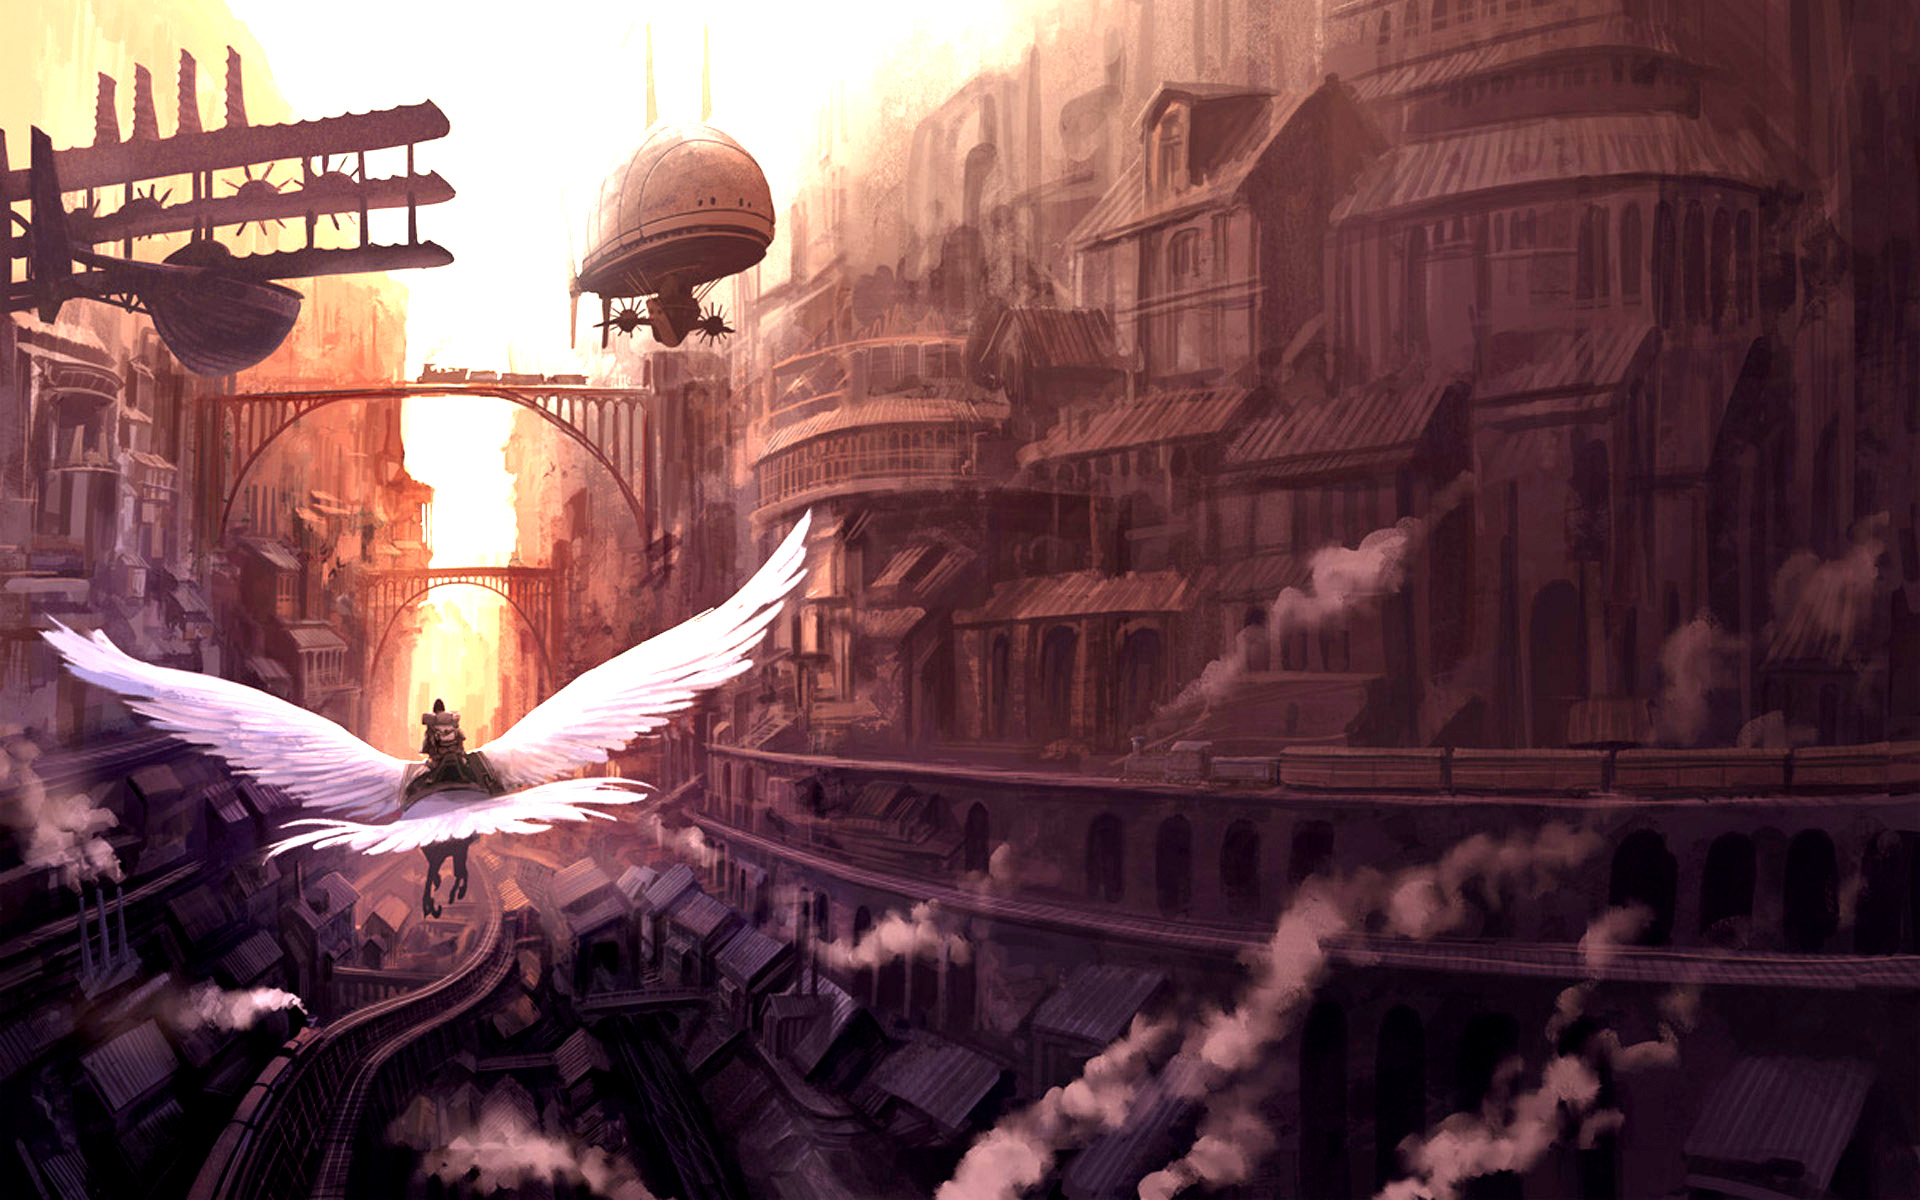
\includegraphics[width=\linewidth]{./images/Annexes/Above-the-city-steampunk-wallpaper.jpg}
\\[-1mm]\citeurl{AboveCityWallpaperSteampunkWallpaper_Matt69ers_sl}
\end{minipage}
\hspace{.02\textwidth}
\begin{minipage}{.49\textwidth}
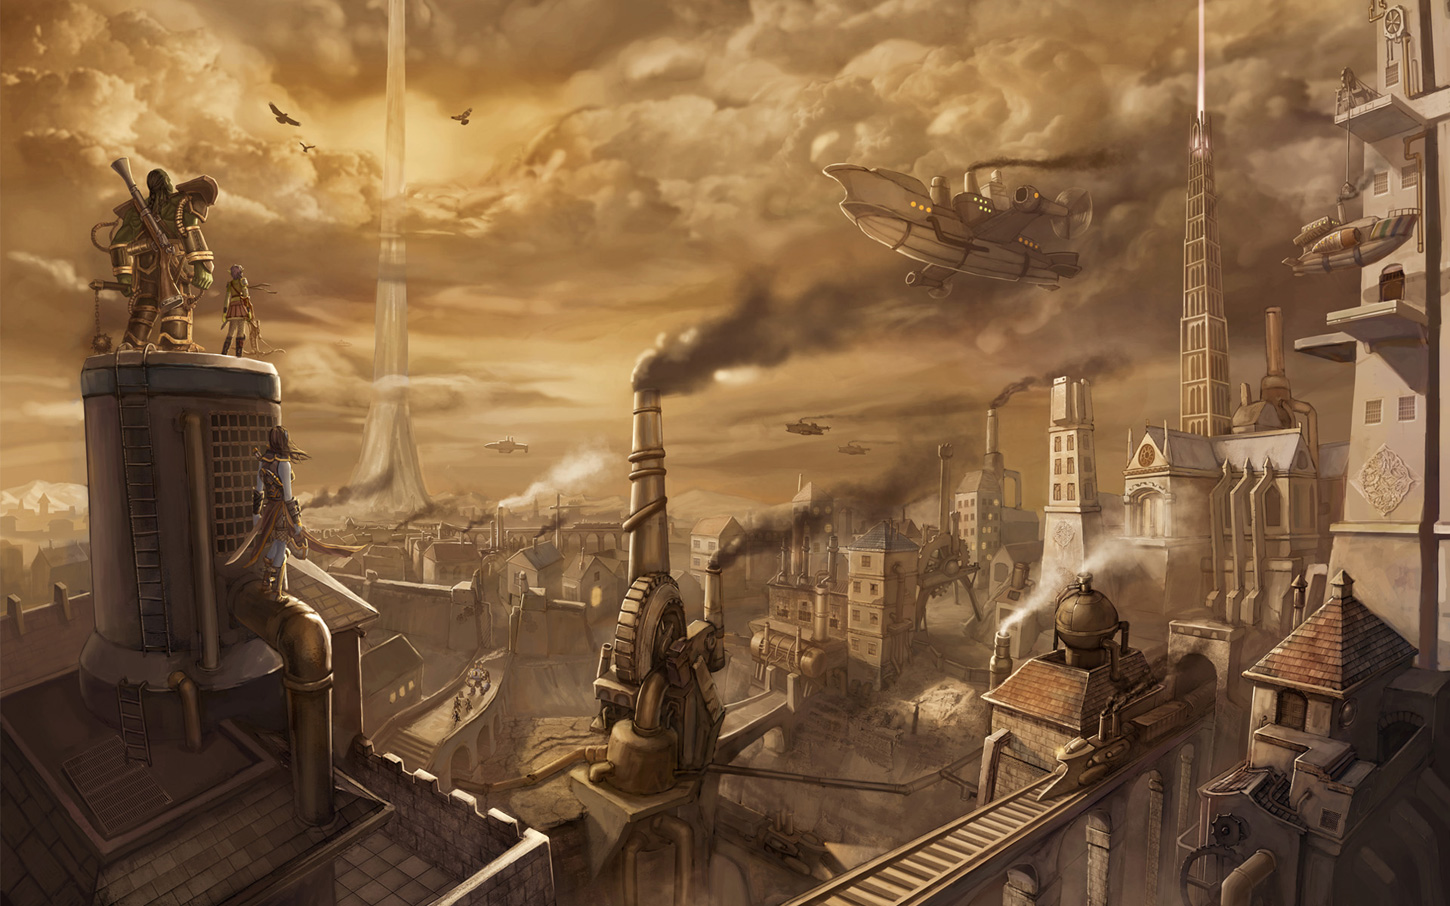
\includegraphics[width=\linewidth]{./images/Annexes/city-of-steam-steampunk.jpg}
\\[-1mm]\citeurl{CityofSteamAcikBetaBasliyor_}
\end{minipage}

\begin{minipage}{.49\textwidth}
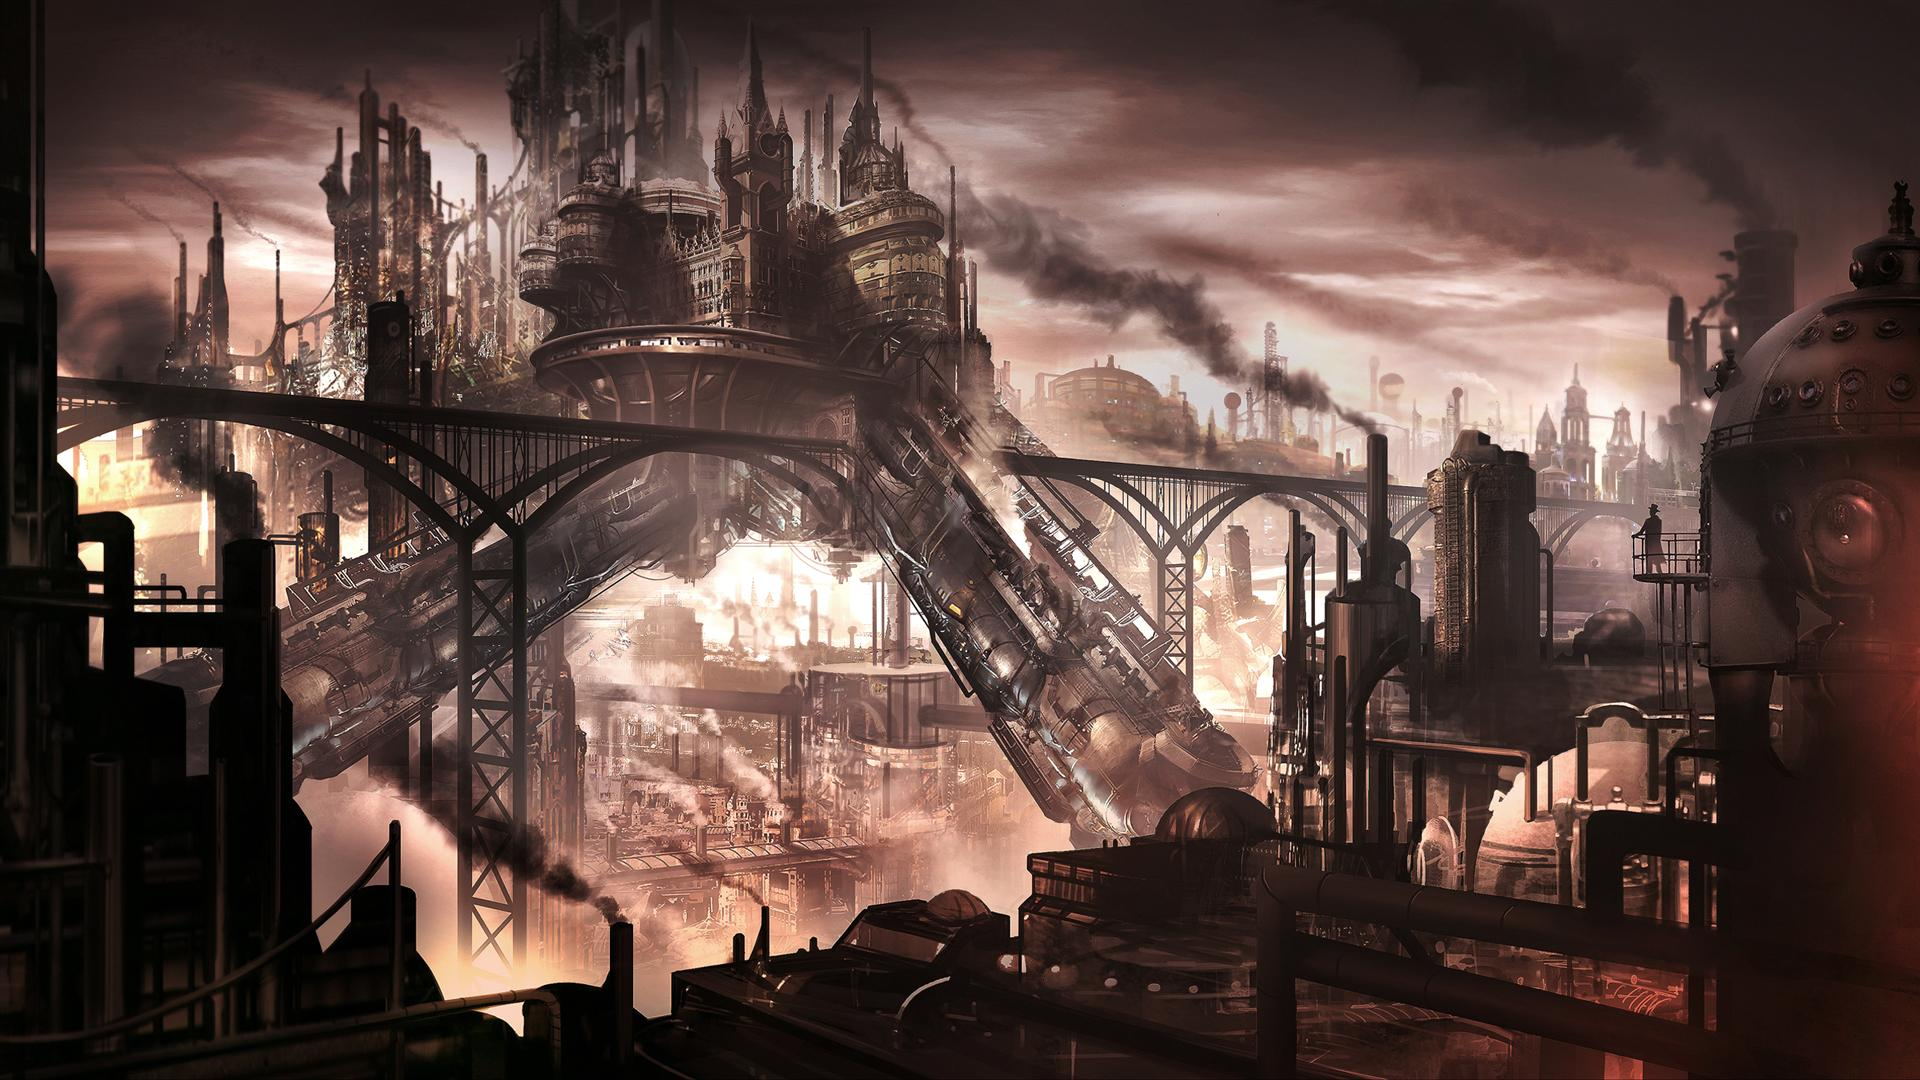
\includegraphics[width=\linewidth]{./images/Annexes/concept_001.jpg}
\\[-1mm]\citeurl{SteampunkTeslapunkonPinterest_}
\end{minipage}
\hspace{.02\textwidth}
\begin{minipage}{.49\textwidth}
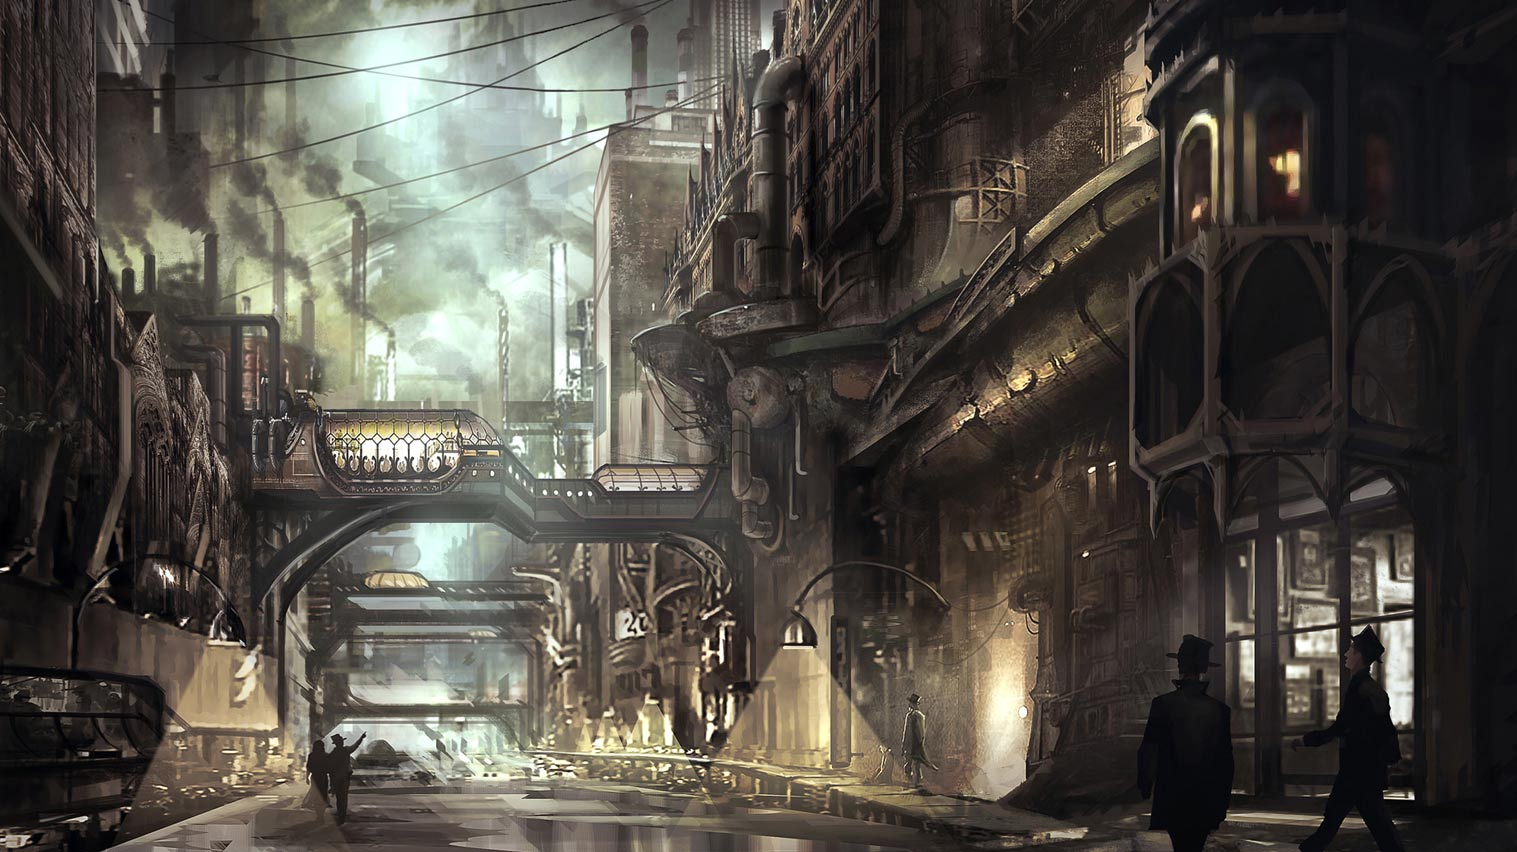
\includegraphics[width=\linewidth]{./images/Annexes/slide-04.jpg}
\\[-1mm]
\url{http://pocketguys.com}
\end{minipage}

\begin{minipage}{\textwidth}
	\begin{minipage}[c]{.49\textwidth}
	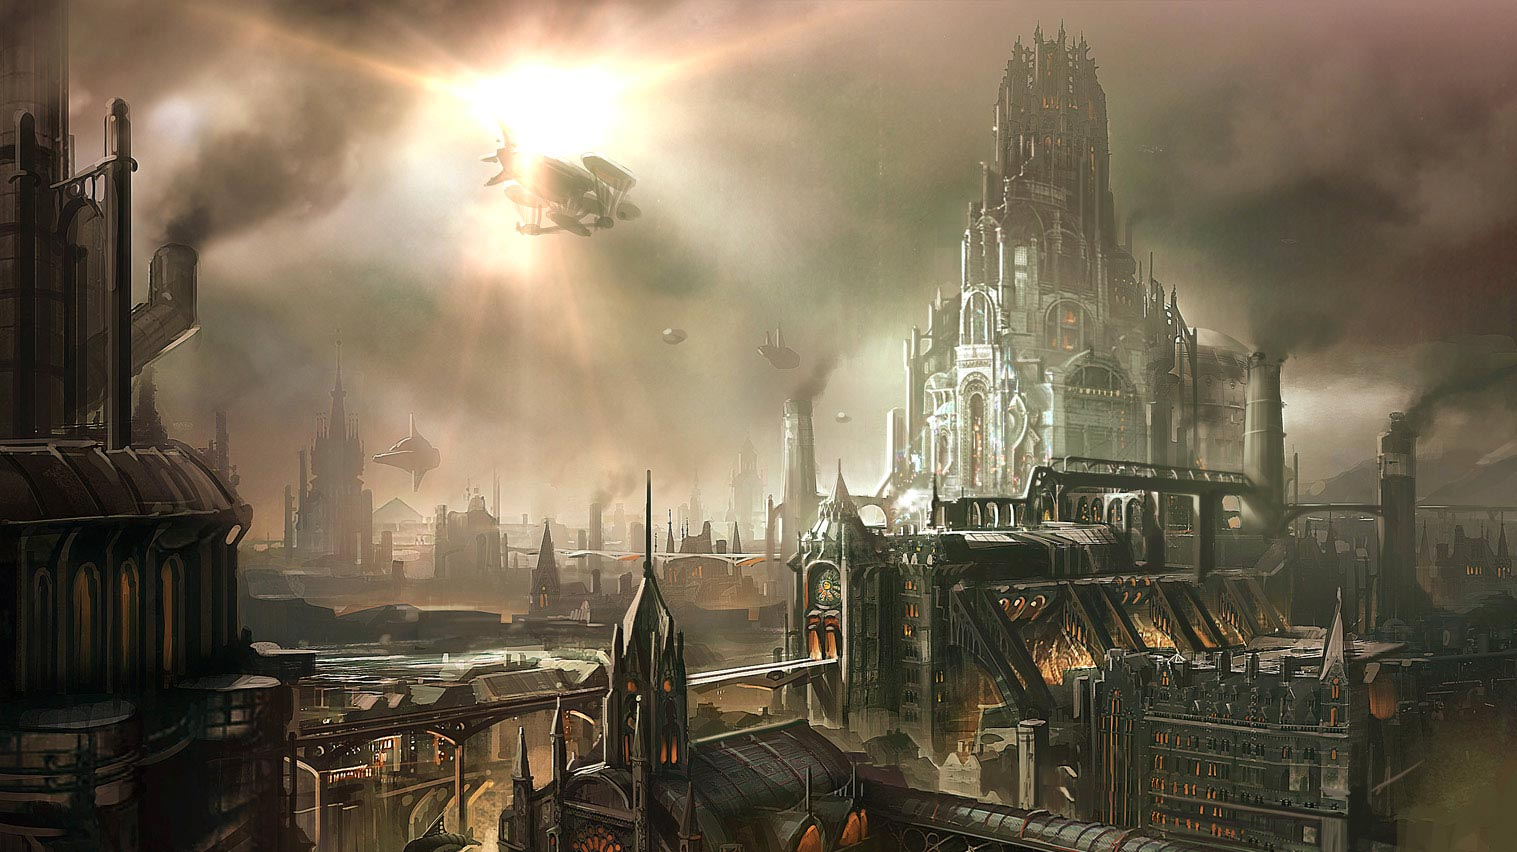
\includegraphics[width=\linewidth, height=4.9cm]{./images/Annexes/slide-02.jpg}
	\\[-1mm]\citeurl{TheScavengers_}
	
	\vspace{2mm}
	
	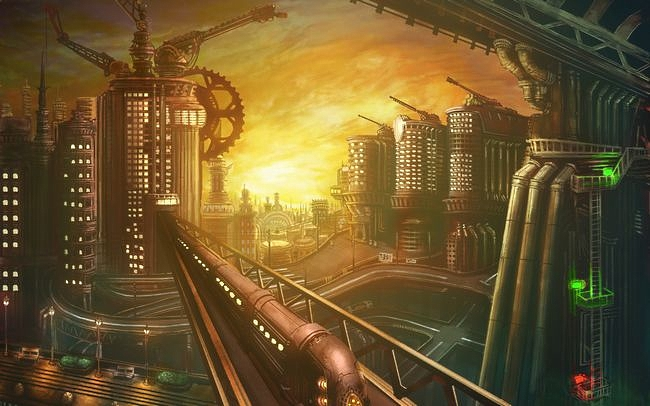
\includegraphics[width=\linewidth, height= 4.9cm]{./images/Annexes/sshot50fd39fccf53c.jpg}
	\\[-1mm]\citeurl{LateAfternoonTrainTravellingThroughaSteampunkCity_}
	\end{minipage}
	\hspace{.02\textwidth}
	\begin{minipage}[c]{.49\textwidth}
	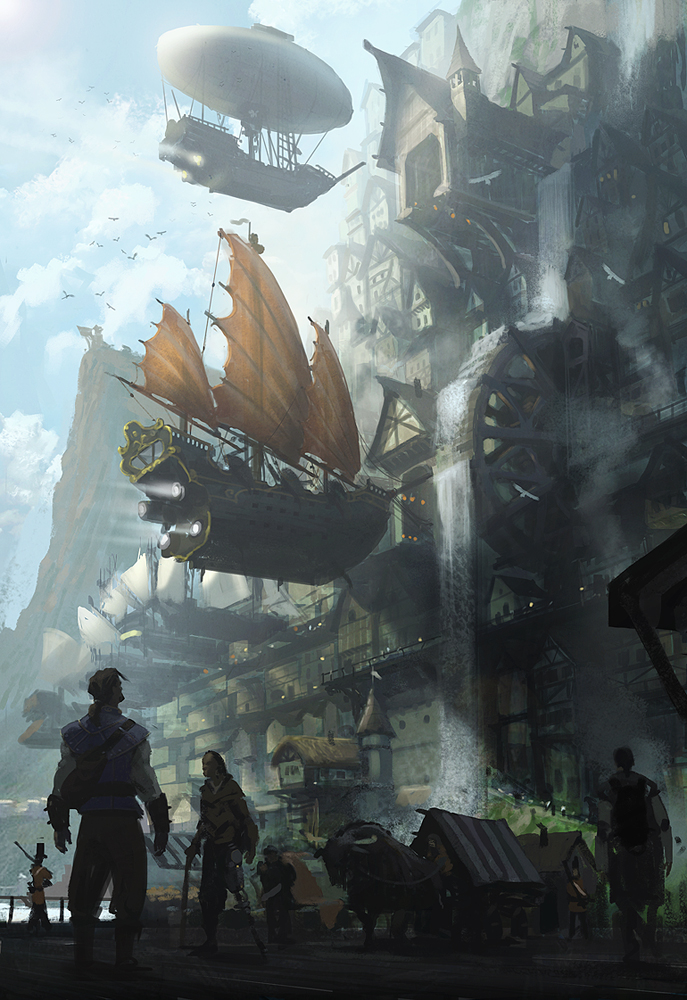
\includegraphics[width=\linewidth]{./images/Annexes/tumblr_mdbq3rCn4e1r4zno6o1_1280.jpg}
	\\[-1mm]\citeurl{SteampunkCityonPinterestSteampunkAirshipSteampunkIllustrationandLadyMechanika_}
	\end{minipage}

\end{minipage}



\chapter{Typographie de ce document}

\hspace*{4.5cm}
\begin{minipage}{\textwidth-4.5cm}
	\setlength{\parskip}{\currentparskip}
	Les points de typographie décrits ci-dessous ignorent la mise en page demandée par le Guide du TM. J'explique dans les paragraphes suivants les raisons qui m'ont poussé à faire ces choix.
	
	\textbf{Police:} La police utilisée dans ce document, Lato, a été choisie pour ses caractères, très adaptés au contenu. Rappelons que le choix d'une police apporte du sens au texte et l'insère dans un contexte culturel et/ou temporel. Si l'utilisation d'un sans-sérifs semblait s'imposer naturellement, l'emploi généralisé de la police Arial la rend banale, inexpressive et peu adaptée. J'ai donc choisi une alternative libre pour ce texte, Lato.
	
	\textbf{Taille de police:} \XeLaTeX, le système utilisé pour la réalisation de ce TM, permet de paramétrer énormément d'aspects de la typographie d'un texte. J'ai utilisé cette flexibilité pour personnaliser ce document et lui donner la forme que je désirais. J'ai, par exemple, aéré les pages pour les rendre plus agréables. Afin que ce document conserve une taille raisonnable, pour avoir un nombre de mots raisonnable par page et pour obtenir un gris typographique plus foncé, le texte est écrit avec du 10pt.
	
	\textbf{Note de bas de page:} Le guide du TM recommande d'utiliser le style de citation décrit par le manuel de style de Chicago. Ce dernier requiert de mettre chaque citation en note de bas de page et dans la bibliographie à la fin du texte. C'est le format généralement utilisé pour les matières littéraires et artistiques. Mais le style de citation est censé changer suivant le style de texte publié : un article de mathématique ne citera pas de la même façon qu'un article économique, qui ne citera pas pareillement qu'un texte littéraire. Pour cette première raison, il semblait plus logique d'utiliser le système \enquote{séquence--citation}\cite{ScientificStyleandFormatOnlineCitationQuickGuide_}, adapté pour les textes scientifiques auquel le mien s’apparente.
\end{minipage}





\chapter*{Déclaration\\\null\hspace*{4.3cm}d'authenticité}
\hspace*{4.5cm}
\begin{minipage}{\textwidth-4.5cm}
	\setlength{\parskip}{\currentparskip}
	\begin{mdframed}[
			linecolor=Grey,
			backgroundcolor=White,
			skipabove=0mm,
			skipbelow=0mm,
			innertopmargin=2mm,
			innerbottommargin=2mm,
			innerleftmargin=2mm,
			innerrightmargin=0mm,
			leftmargin=0mm,
			rightline=false,
			topline=false,
			bottomline=false,
			linewidth=1mm
		]
		PLAGIAIRE\\
		\lbrack plaЗјєR\rbrack\ n. -- plagiere 1584; lat. plagiarius \enquote{celui qui vole les esclaves d’autrui}, du gr. Plagios
		\enquote{oblique, fourbe} $\blacklozenge$ Personne qui pille ou démarque les ouvrages des auteurs.
		
		PLAGIER\\
		\lbrack plaЗјє\rbrack\ v.tr. -- 1801; de plagiat 1. Copier (un auteur) en s’attribuant indûment des passages de son
		oeuvre. $\rightarrow$ \textbf{imiter, piller}.
		
		\hfill (Petit Robert I - éd. 1996)
	\end{mdframed}
	
	\vspace*{1cm}
\end{minipage}



\chapter*{Bibliographie}
\sloppy
\hspace*{4.2cm}
\begin{minipage}{\textwidth-4.2cm}
	\printbibliography[notkeyword=image, heading=none]
\end{minipage}



\chapter*{Iconographie}

\hspace*{4.2cm}
\begin{minipage}{\textwidth-4.2cm}
	\printbibliography[keyword=image, heading=none]
\end{minipage}



%\printindex
%\newpage
%
%\listoffigures
%
%\listoftables
%
%\begingroup
%\let\clearpage\relax
%\lstlistoflistings
%\endgroup



